\renewcommand{\assert}[1]{\ensuremath{\{\;#1\;\}}}

\section{Algorithmen: Hoare-Kalkül}

\subsection{Algorithmen}
\begin{frame}
	\begin{block}{Definition}
		Über die Eigenschaften von Algorithmen:
		\begin{itemize}[<+->]
			\item Eine endliche Beschreibung...
			\item ...aus elementaren Aussagen...
			\item ... die deterministisch ausgeführt werden.\\
				(Manchmal auch gemischt mit (Pseudo-)Zufallselementen)
			\item Eine endliche Eingabe gibt endliche Ausgabe...
			\item in endlich vielen Schritten.
			\item Das funktioniert für beliebig große Eingaben und
			\item ist nachvollziehbar bzw. verständlich
		\end{itemize}
	\end{block}
	\pause
	Woher wissen wir, ob ein Algorithmus korrekt ist?
\end{frame}

\begin{frame}{Korrektheit}
	Einige Algorithmen haben besonders hohe Anforderungen an die Korrektheit:
	Banking-Server, Airbag-Steuerprogramm, Herzschrittmacher, ...
	\bigskip

	\pause
	Wie können wir die Korrektheit beweisen?
	\begin{itemize}[<+->]
		\item Testen? Was, wenn wir einen Sonderfall vergessen?
		\item Alle Eingaben testen? Oft nicht möglich.
		\item Formal beweisen: Hoare-Kalkül
	\end{itemize}
	
	\pause
	\begin{block}{In der Praxis}
		Theoretisch müsste die komplette Werkzeugkette bewiesen werden:
		Programm, Compiler, Prozessor...\\
		Oft wird bei Compilern nur “Proven in use” benutzt: Compiler, bei
		denen seit Jahren keine Fehler gefunden wurden.
	\end{block}
	
\end{frame}

\subsection{Hoare-Kalkül}
\begin{frame}{Das Hoare-Kalkül}
	\begin{block}{Definition}
		Ein \emph{Hoare-Tripel} ist ein Tupel $(\{P\}\ S\ \{Q\})$ mit einem Programmstück $S$ und prädikatenlogischen \emph{Zusicherungen} $P,Q$.
	\end{block}
	\pause
	$P = $ Bedingung vor der Ausführung \\
	$Q = $ Zusicherung nach der Ausführung\\
	$S = $ Programmstück
	
	\pause
	\bigskip
	Dabei: Wir betrachten nur \enquote{relevante} Interpretationen:
	\begin{itemize}[<+->]
		\item Fester Grundbereich (explizit angegeben oder implizit ableitbar)
		\item Funktionen und Relationen \enquote{wie üblich} interpretiert.
		\item Konstanten beliebig, als \enquote{Eingabe} des Programms.\\
		Muss also für alle Möglichkeiten = Eingaben gelten.
	\end{itemize}
\end{frame}

%TODO
\begin{frame}{Das Hoare-Kalkül}
	\begin{block}{Definition}
		Ein Hoare-Tripel $\htr{P}{S}{Q}$ ist gültig, wenn für jede relevante Interpretation und jede Variablenbelegung $\beta$ gilt:\\
		Wenn vor der Ausführung $\val_{D,I,\beta}(P)=\W$ ist und wenn die Ausführung von $S$ für $I$ und $\beta$ endet und hinterher Variablenbelegung $\beta'$ vorliegt, dann gilt am Ende $\val_{D,I,\beta'}(Q)=\W$.
	\end{block}

	\pause
	\begin{block}{Hoare-Kalkül}
		Das \emph{Hoare-Kalkül} definiert Regeln, wie gültige \emph{Hoare-Tripel} schrittweise abgeleitet werden können.
	\end{block}
\end{frame}


\begin{frame}{HT-A}
	\begin{block} {Axiom HT-A}
		$$ \{\sigma_{\text{x/E}} (Q)\} \ x \leftarrow E \ \{Q\} $$
	\end{block}
	\pause
	Nach einer Zuweisung gilt jede Aussage für die Variable, welche vorher für die linke Seite der Zuweisung galt.
	\begin{itemize}
		\item $\sigma_{\text{x/E}} (Q) $ ist die Aussage, die dadurch entsteht, dass man in Q jedes freie Vorkommen von x durch E ersetzt.
		\item Achtung: $\sigma_{\text{x/E}}$ muss kollisionfrei sein!
	\end{itemize}
	\vspace{2em}
	\begin{Beispiel}
		$\{ x + 1 = 43\} \ y := x + 1\ \{y = 43 \}.$
	\end{Beispiel}
	
\end{frame}

\begin{frame}{HT-E}
	\begin{block}{Regel HT-E}
		Wenn $\{P\}\ S\ \{Q\}$ gültig ist, dann auch $\{P'\}\ S\ \{Q'\}$ mit $P' \implies P$ und $Q \implies Q'$.
	\end{block}
	\pause
	Vorbedingungen können stärker, Nachbedingungen können schwächer werden.

\end{frame}

\begin{frame}{HT-S}
	\begin{block}{Regel HT-S}
		Wenn $\{P\}\ S_1\ \{Q\}$ und $\{Q\}\ S_2\ \{R\}$ gültig sind, dann auch $\{P\}\ S_1 S_2\ \{R\}$. 
	\end{block}
	\pause
	Hoare-Tripel können transitiv zusammengefasst werden.
\end{frame}

\begin{frame}
	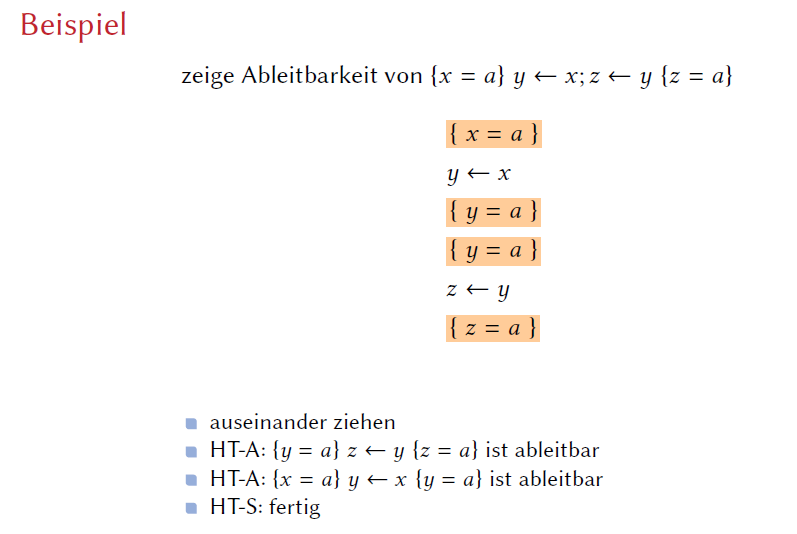
\includegraphics[scale=0.5]{hoare/bsp1}
\end{frame}

\begin{frame}{HT-I}
	\begin{minipage}{0.4\linewidth}
		\begin{align*}
			&\{ P \} \\
			& \textbf{if } B \\
			& \textbf{then} \\
			&\hspace{2em} \{ P \wedge B \} \\
			&\hspace{2em} S_1 \\
			&\hspace{2em} \{ Q \}\\
			&\textbf{else} \\
			&\hspace{2em} \{ P \wedge \neg B \} \\
			&\hspace{2em} S_2 \\
			&\hspace{2em} \{ Q \}  \\
			&\textbf{fi}\\
			&\{Q \}
		\end{align*}
	\end{minipage}
	\begin{minipage}{0.55\linewidth}
		\begin{block}{Regel HT-I}
			$\textbf{if } B\text{ } \textbf{then } S_1 \textbf{ else } S_2 \textbf{ fi}$
			\vspace{1em}
			\begin{itemize}
				\item Wenn $\{ P \wedge B \} S_1 \{ Q \}$ gültig 
				\item und $\{ P \wedge \neg B \} S_2 \{ Q \}$ gültig
				\item dann auch $\{ P \} \textbf{ if } B \textbf{ then } S_1 \textbf{ else } S_2 \textbf{ fi} \{ Q \} $ gültig
			\end{itemize}
		\end{block}
%		\emph{HT4 : } $\textbf{if } B\text{ } \textbf{then } S_1 \textbf{ else } S_2 \textbf{ fi}$
%		\begin{itemize}
%			\item Wenn $\{ P \wedge B \} S_1 \{ Q \}$ gültig 
%			\item Wenn $\{ P \wedge \neg B \} S_2 \{ Q \}$ gültig
%			\item dann auch $\{ P \} \textbf{ if } B \textbf{ then } S_1 \textbf{ else } S_2 \textbf{ fi} \{ Q \} $ gültig
%		\end{itemize}
	\end{minipage}
\end{frame}

\begin{frame}{Beispiel $\vert x \vert$}
	\vspace{-10mm}
	\begin{align*}
		&\{ x \in\R\} \\
		&\textbf{if } x < 0 \\
		&\textbf{then } \\
		&\hspace{2em} \{ \only<6->{ z\in\R\wedge x < 0 } \} \\
		&\hspace{2em} \{ \only<5->{ -x = \vert x \vert } \} \\
		&\hspace{2em}  z \leftarrow -x   \\
		&\hspace{2em} \{ \only<2->{ z = \vert x \vert } \} \\
		&\textbf{else} \\
		&\hspace{2em} \{ \only<4->{ z\in\R\wedge x\geq 0 } \} \\
		&\hspace{2em} \{ \only<3->{ x = \vert x \vert } \} \\
		&\hspace{2em} z \leftarrow x \\
		&\hspace{2em} \{ \only<2->{ z = \vert x \vert } \} \\
		&\textbf{fi} \\
		&\{ z = \vert x \vert \} 
	\end{align*}
\end{frame}

\begin{frame}{Aufgabe}
	\vspace{-10mm}
	  \begin{alignat*}{2}
	&\assert{x=a \land y=b}  \\
	&\kw{if } x>y  \\
	&\kw{then } \\
	&&&\assert{ \dots\ } \\
	&&& z \gets y  \\
	&&&\assert{ \dots\ } \\
	&\kw{else } \\
	&&&\assert{ \dots\ } \\
	&&& z \gets x  \\
	&&&\assert{ \dots\ } \\
	&\kw{fi } \\
	&\assert{z=\min(a,b)}
	\end{alignat*}
\end{frame}

\begin{frame}{Lösung}	
	\vspace{-15mm}
	\begin{alignat*}{2}
	&\assert{x=a \land y=b}  \\
	&\kw{if } x>y  \\
	&\kw{then } \\
	&&&\assert{x=a \land y=b \land x>y} \\
	&&&\assert{y=\min(a,b)} \\
	&&& z \gets y  \\
	&&&\assert{z=\min(a,b)} \\
	&\kw{else } \\
	&&&\assert{x=a \land y=b \land  \lnot (x>y)} \\
	&&&\assert{x=\min(a,b)} \\
	&&& z \gets x  \\
	&&&\assert{z=\min(a,b)} \\
	&\kw{fi } \\
	&\assert{z=\min(a,b)}
	\end{alignat*}
\end{frame}


%TODO: Lösung!!!
%\begin{frame}
%	\frametitle{Jetzt seid ihr dran}
%	\begin{align*}
%		& z \leftarrow x + y \\
%		& z \leftarrow z / 2 \\
%		&\textbf{if } x\ mod\ 2 = 0 \\
%		&\textbf{then } \\
%		&\hspace{2em} y \leftarrow x + x \\
%		&\hspace{2em} y \leftarrow y / 4 \\
%		&\textbf{else} \\
%		&\hspace{2em} y \leftarrow x - 1 \\
%		&\hspace{2em} y \leftarrow y / 2 \\
%		&\textbf{fi} \\
%		& z \leftarrow z * y \\
%		&\{ z = div_2(a) * (a+b)/2 \} 
%	\end{align*}
%\end{frame}

\begin{frame}
	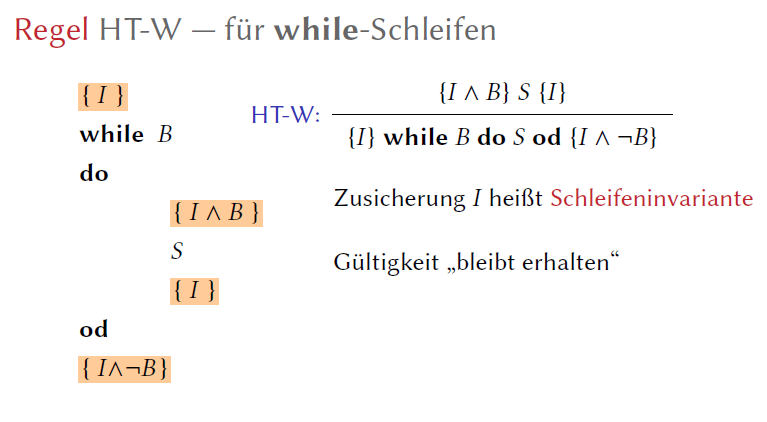
\includegraphics[scale=0.5]{hoare/htw}
\end{frame}

\subsection{Schleifeninvarianten}
\begin{frame}{Schleifeninvarianten}
	\begin{block}{}
		Schleifeninvarianten ... 
		\begin{itemize}
			\item sind Aussagen, die bei jedem Schleifendurchgang gültig sind
			\item helfen, die Korrektheit eines Programmes zu beweisen
			\item muss man ebenfalls beweisen
			\item garantieren nicht die Korrektheit des Programms:\pause \\
			 Terminierung der Schleife muss zusätzlich gezeigt werden!
		\end{itemize}
	\end{block}
\end{frame}
	
\begin{frame}{Beispiel}
	\begin{minipage}{0.49\linewidth}
	\begin{align*}
		&\assert{x=a \land y=b}  \\
		&\assert{ \dots\ } \\
		&\kw{while } \; y\not=0  \\
		&\kw{do } \\
		&\qquad\assert{ \dots } \\
		&\qquad y \gets y-1 \\
		&\qquad\assert{ \dots } \\
		&\qquad x \gets x+1 \\
		&\qquad\assert{ \dots\ } \\
		&\kw{od } \\
		&\assert{ \dots\ } \\ \pause
		&\assert{x=a+b} \\
	\end{align*}
	\end{minipage} \pause
	\begin{minipage}{0.5\linewidth}
		\begin{block}{Wertetabelle für a=3 und b=4}
			\centering
			\begin{tabular}{ccc}	 
				i & x & y \\
				0 & 3 & 4 \\
				1 & 4 & 3 \\
				2 & 5 & 2 \\
				3 & 6 & 1 \\
				4 & 7 & 0 \\
			\end{tabular}
		\end{block}
		\pause
		Schleifeninvariante : $$ x_i + y_i = a + b $$ 
	\end{minipage}
\end{frame}

\begin{frame}{Beispiel}
	\vspace{-5mm}
	\begin{align*}
		&\assert{x=a \land y=b }  \\
		&\assert{x+y=a+b }  \\
		&\kw{while } \; y\not=0  \\
		&\kw{do } \\
		&\qquad\assert{x+y=a+b \land y\not=0 }  \\
		&\qquad\assert{x+1+y-1=a+b } \\
		&\qquad y \gets y-1 \\
		&\qquad\assert{x+1+y = a+b} \\
		&\qquad x \gets x+1 \\
		&\qquad\assert{x+y = a+b} \\
		&\kw{od } \\
		&\assert{x+y = a+b \land (y=0) } \\
		&\assert{x=a+b} \\
	\end{align*}
\end{frame}

\begin{frame}{SIV mit Vollständiger Induktion}
	Wir zeigen mit vollständiger Induktion die Gültigkeit der Schleifeninvariante. Dabei sei $i$ die Anzahl der bisherigen Schleifendurchläufe.\\
	
	\emph{Behauptung}: $$ \forall\ i \in \{0,b\} : x_i + y_i = a+b $$ \pause
	\begin{block}{Induktionsanfang}
		Für $i=0$ gilt $ x_0+y_0 = a+b $ nach Vorbedingung
	\end{block} \pause 
	\begin{block}{Induktionsvorrausetzung}
		Für ein beliebig aber festes $i\in \{0,b\}$ gelte die Behauptung
	\end{block}
\end{frame}

\begin{frame}{SIV mit Vollständiger Induktion}
	\begin{block}{Induktionsschluß}
		Zu zeigen $$ x_{i+1} + y_{i+1} = a+b $$ \pause
		\begin{align*}
		x_{i+1}+y_{i+1} &= x_i +1 + y_i -1 \\
		&= x_i + y_i \\
		&\overset{IV}{=} a+b
		\end{align*}
	\end{block}
\end{frame}

\begin{frame} {Weitere Beispiele}
	Weitere Beispiele findet ihr hier: Übung 8, WS 15/16
\end{frame}